\documentclass{article}
\usepackage[utf8]{inputenc}
\usepackage{listings}
\usepackage{color} 
\usepackage{hyperref}
\usepackage{float}
\usepackage{subcaption}

\hypersetup{
    colorlinks=true, %set true if you want colored links
    linktoc=all,     %set to all if you want both sections and subsections linked
    linkcolor=blue,  %choose some color if you want links to stand out
}

%\usepackage{titling}
\usepackage{graphicx}
%\usepackage{titlepic}

\lstset{
	frame=tb, % draw a frame at the top and bottom of the code block
   	tabsize=4, % tab space width
   	showstringspaces=false, % don't mark spaces in strings
    numbers=left, % display line numbers on the left
    commentstyle=\color{red}, % comment color
    keywordstyle=\color{blue}, % keyword color
    stringstyle=\color{green} % string color
}


\title{\vspace*{\fill} \textbf{COP 290 Assignment 2}
	  \\ {\Large \textbf{Complaint Management System}}
	  % \\  \vspace{3mm} \includegraphics{ddlogo.png}}
}
\author{
	\vspace{5mm} 
\includegraphics[width=5cm]{logo.png} \\
	 \textbf{Aditi}\\
	2014CS10205 \vspace{2mm} \\
	\textbf{Ayush Bhardwaj}\\ 
	2014CS10091 \vspace{2mm} \\
	\textbf{Nikhil Gupta}\\ 
	2014CS50462 \vspace{2mm}
}
\date{\vspace{3mm} \textbf{March 2016} \vspace*{\fill}}

\begin{document}
	\maketitle

	\newpage

	\tableofcontents

	\newpage

	\section{Objectives}
		Design an App which is :
		\begin{itemize} 
			\item Complaint Management System for IIT Delhi
			\item The Users of the App would be the people of the institute such as faculties, students, and institute employees
			\item Addresses three levels of complaints: 
				\begin{enumerate}
					\item Individual Complaint 
					\item Hostel-level Complaint
					\item Institute-level complaint
				\end{enumerate}
			\item The users can submit their grievance to the the concerned authorities
		\end{itemize}
		%\begin{figure}[H]
          %\centering
            %\includegraphics[width=1.0\linewidth]{gameplay.png}
        %\end{figure}
	\section{Overall Design}
		%The game which we will build is space invaders. It involves the player controlling a space ship and shooting down aliens. The aliens will fight back with bullets and missiles. The player has a limited number of lives and has to score the maximum in them.
		TODO:  Add a basic description of main classes as in previous design doc 
		Different layouts
		\begin{enumerate}
			\item The server side will be programmed in Web2py ~\cite{Web2py_Basics}
			\item The android app will be made using Java
			\item The app would be extended to other phones as well as web clients
			\item Volley will be used to send requests and receive responses
			\item Shared Preferences will be used to maintain the feature of Persistent login 
			\item Doxygen will be used to create HTML documentation of the entire code base.
			\item Users can select their preferred topics.Only complaints related to selected topics will be visible to the user.
			\item The entire code will be split up in multiple files to ensure modularity in code. 
		\end{enumerate}
	\section{User Interface}
	TODO Add info \\
	    \begin{figure}[H]
      \centering
      \begin{subfigure}{.4\textwidth}
          \centering
          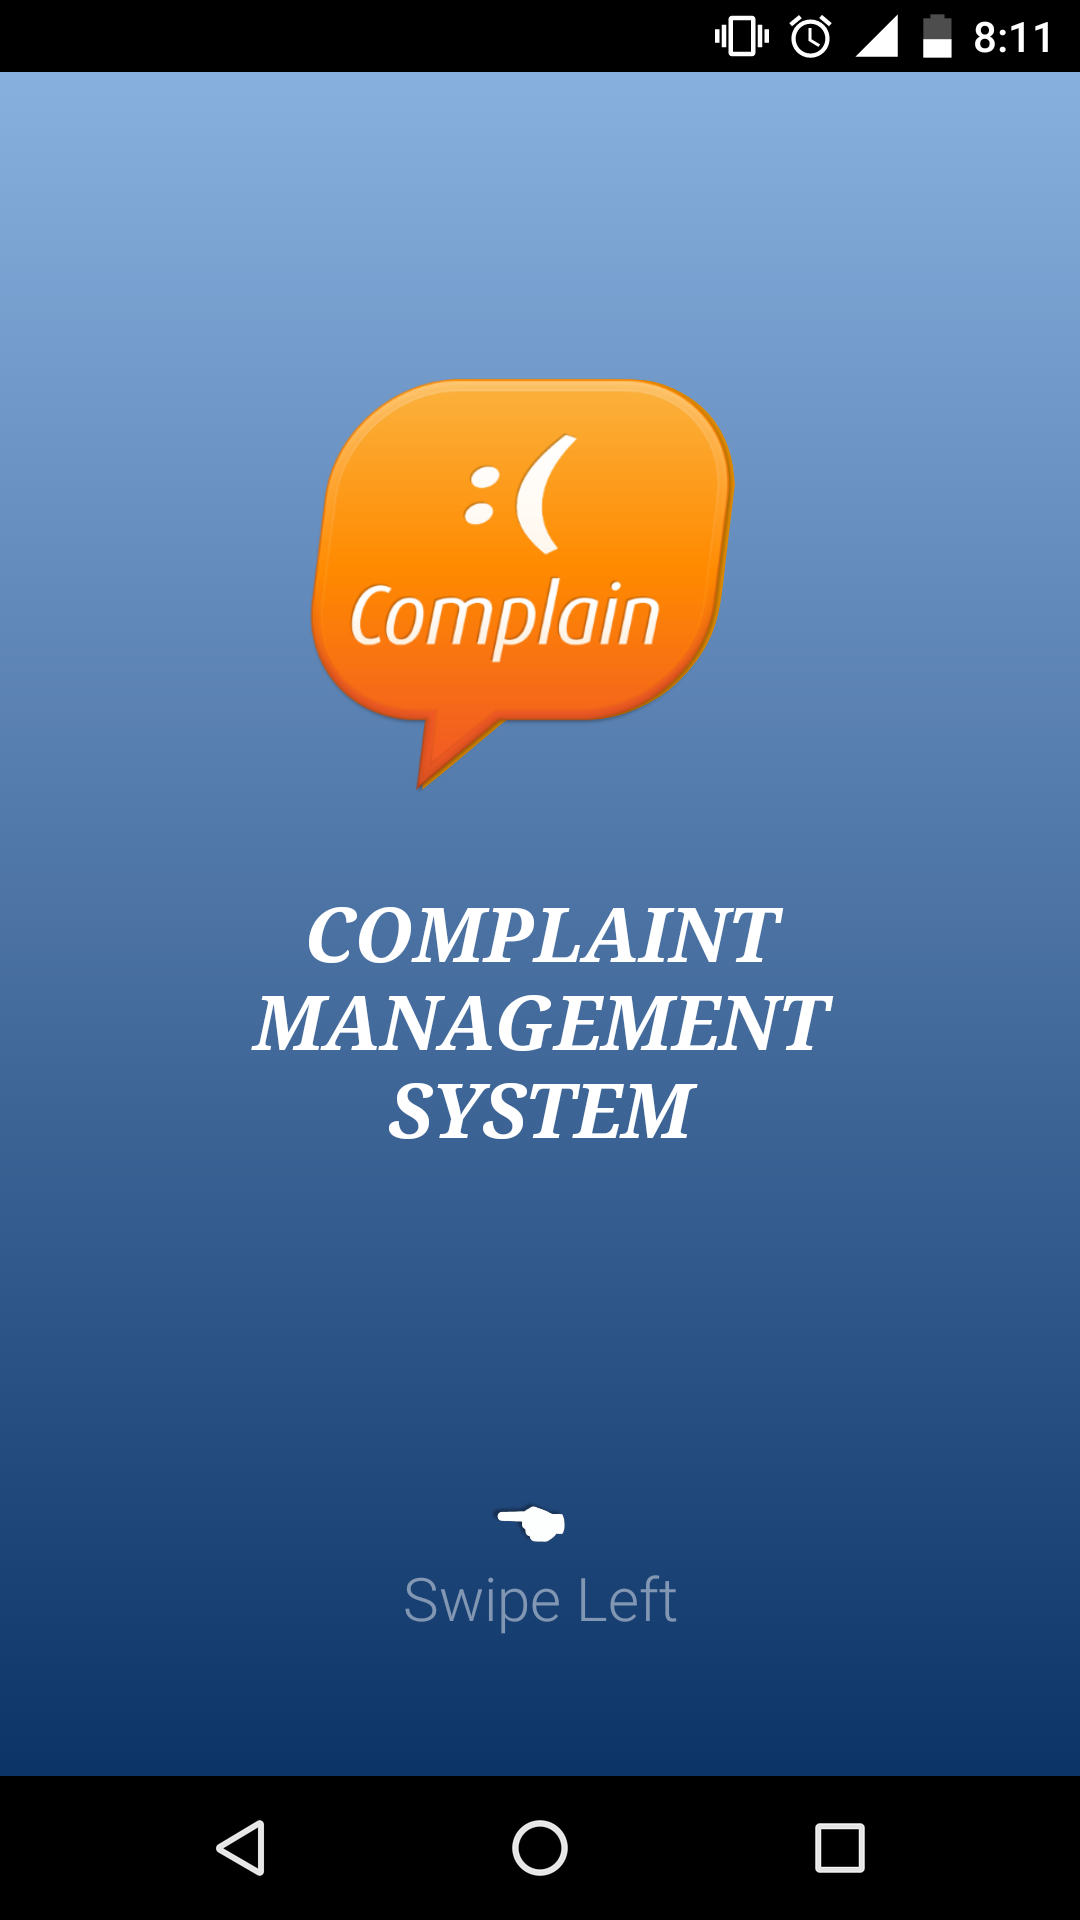
\includegraphics[width=0.9\linewidth]{splash.png}
          \caption{Splash Screen}
          \label{fig:sub1}
      \end{subfigure}%
      \begin{subfigure}{.4\textwidth}
          \centering
          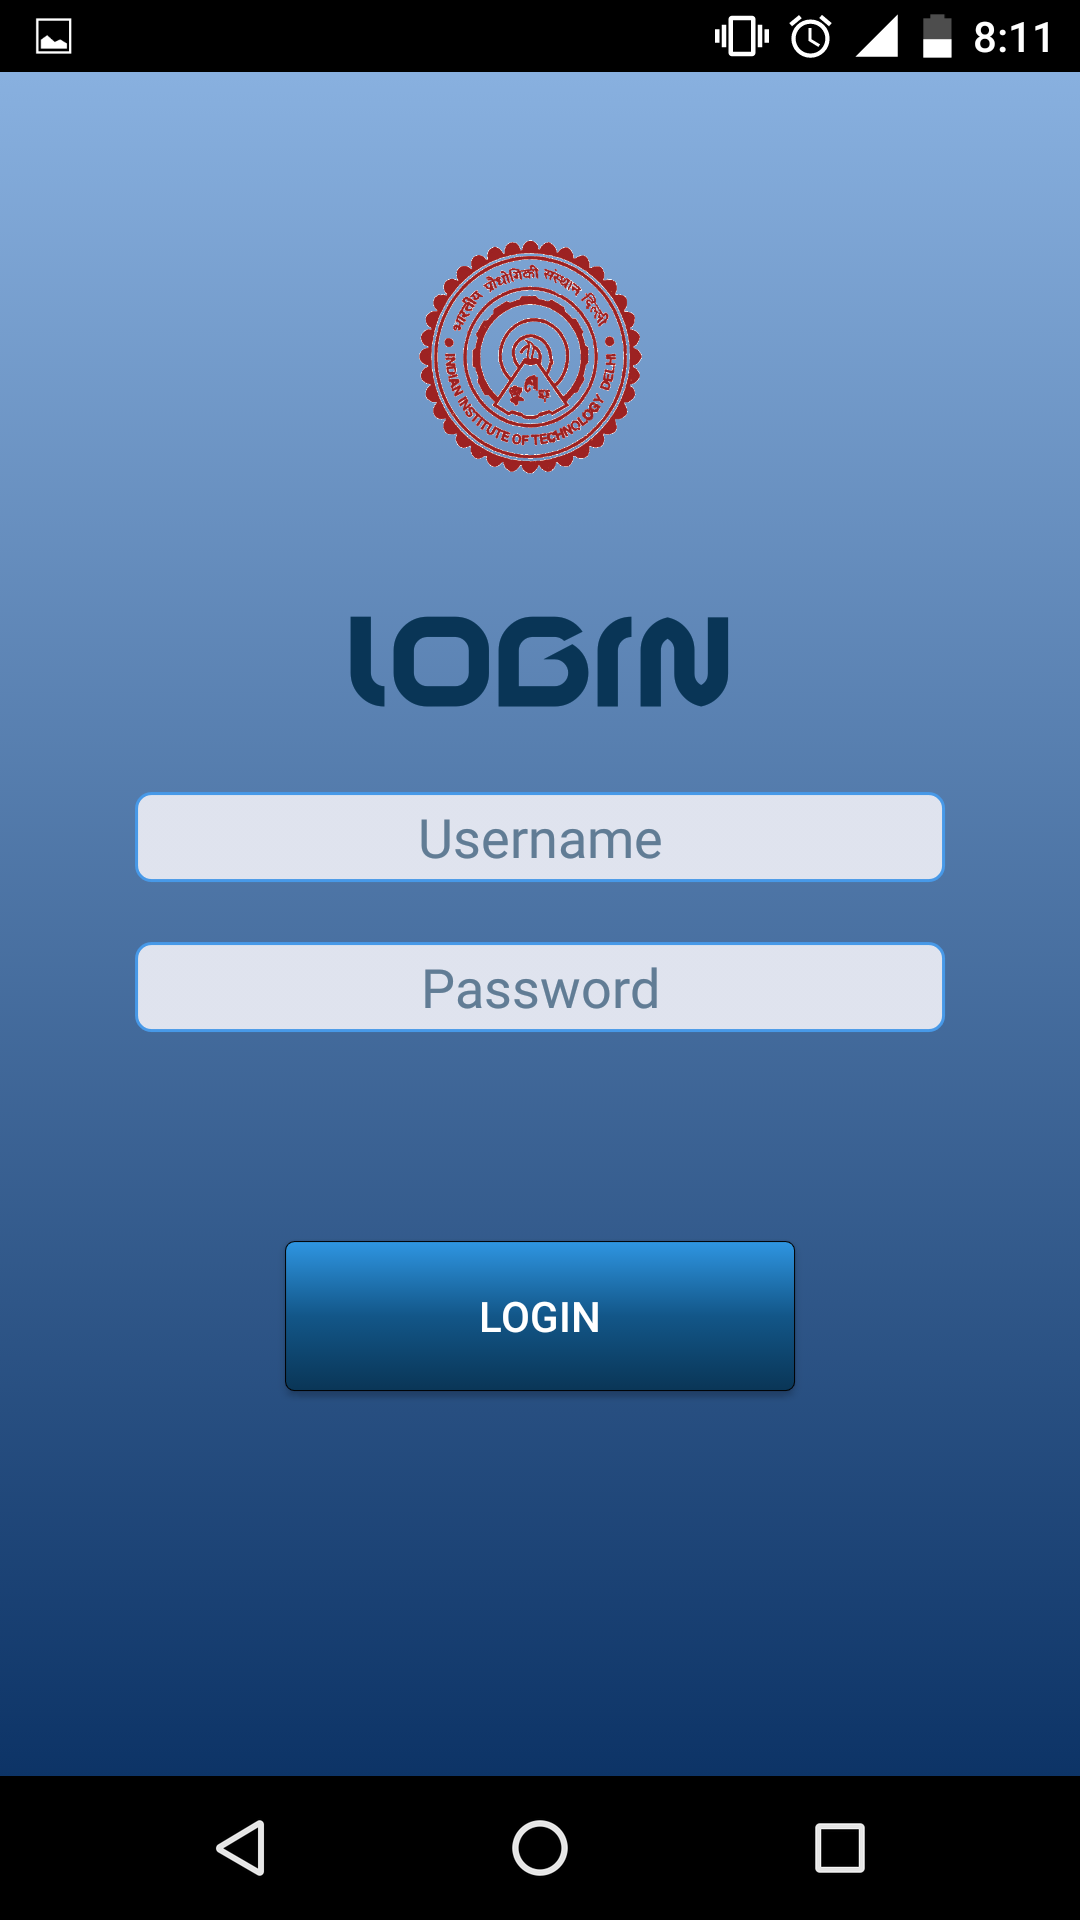
\includegraphics[width=0.9\linewidth]{loginui.png}
          \caption{Login Page}
          \label{fig:sub2}
      \end{subfigure}
      % \caption{3D reconstruction}
      \label{figstart}
    \end{figure}

	    \begin{figure}[H]
      \centering
      \begin{subfigure}{.4\textwidth}
          \centering
          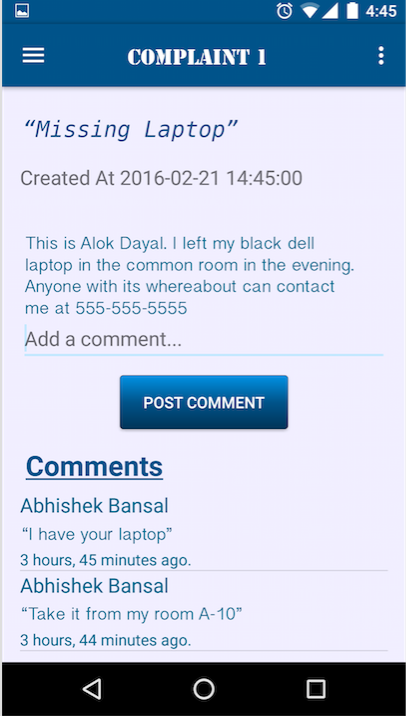
\includegraphics[width=0.9\linewidth]{insidecomplaint.png}
          \caption{Complaint Information UI}
          \label{fig:sub1}
      \end{subfigure}%
      \begin{subfigure}{.4\textwidth}
          \centering
          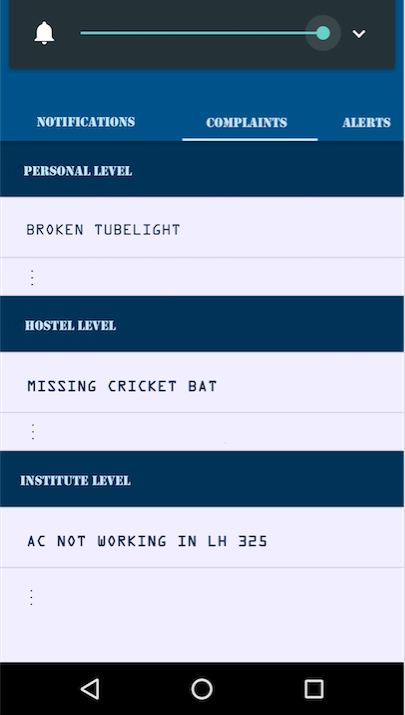
\includegraphics[width=0.9\linewidth]{listcomplaints.png}
          \caption{Complaints List View}
          \label{fig:sub2}
      \end{subfigure}
      % \caption{3D reconstruction}
      \label{figstart}
    \end{figure}


	    \begin{figure}[H]
      \centering
      \begin{subfigure}{.5\textwidth}
          \centering
		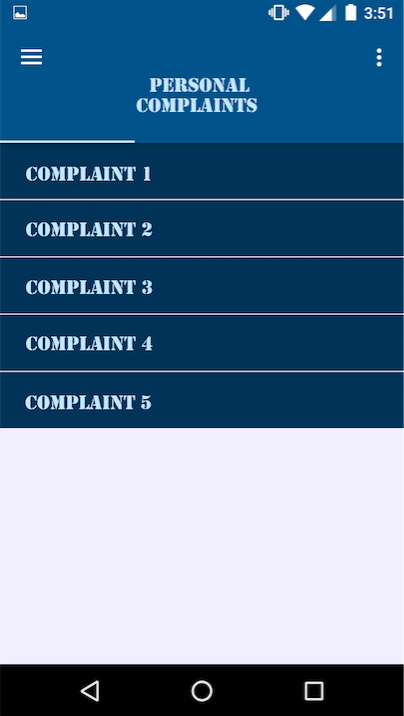
\includegraphics[width=0.9\linewidth]{test1complaints.png}
          \caption{Complaint Type Screen}
          \label{fig:sub1}
      \end{subfigure}%
      % \caption{3D reconstruction}
      \label{figstart}
    \end{figure}

    	\subsection{Visioned Pages}
    		\subsubsection{Splash Screen}
    			\begin{itemize}
    			\item This is the first screen that is displayed on the starting of the app.
    			\item It has been made dynamic and interactive by adding animations and gesture recognitions
    			\end{itemize}
    		\subsubsection{Login Screen}
    			\begin{itemize}
    			\item The login page requests for the user's username and password and validates the login.
    			\item It is displayed only after left swiping the splash screen.
    			\end{itemize}
    		\subsubsection{Complaint List Screen}
    			\begin{itemize}
    			\item This screen is a tabbed activity that contains the following tabs:
    				\begin{enumerate}
    					\item Notifications (Displays new complaints)
						\item Complaints (Displays all the complaints, sorted by their types)
						\item Alerts (Displays the complaints important to the user
						)
					\end{enumerate}
				\item The tabs contain information using ListViews
				\end{itemize}
			\subsubsection{Complaint Type Screen}    
				\begin{itemize}	
				\item This screen lists all complaints of the same type in an ExplandableList type.
				\item Clicking on a particular complaint will list some basic detains about the complaint.
				\item Appyling the sliding gesture on the complaint will open up the detailed complaint information screen.
				\end{itemize}
			\subsubsection{Complaint Information Screen}
				\begin{itemize}
				\item This screen contails all the indepth details of the complaint.
				\item It allows the user to add comments to the thread of the complaint.
				\end{itemize}

		% 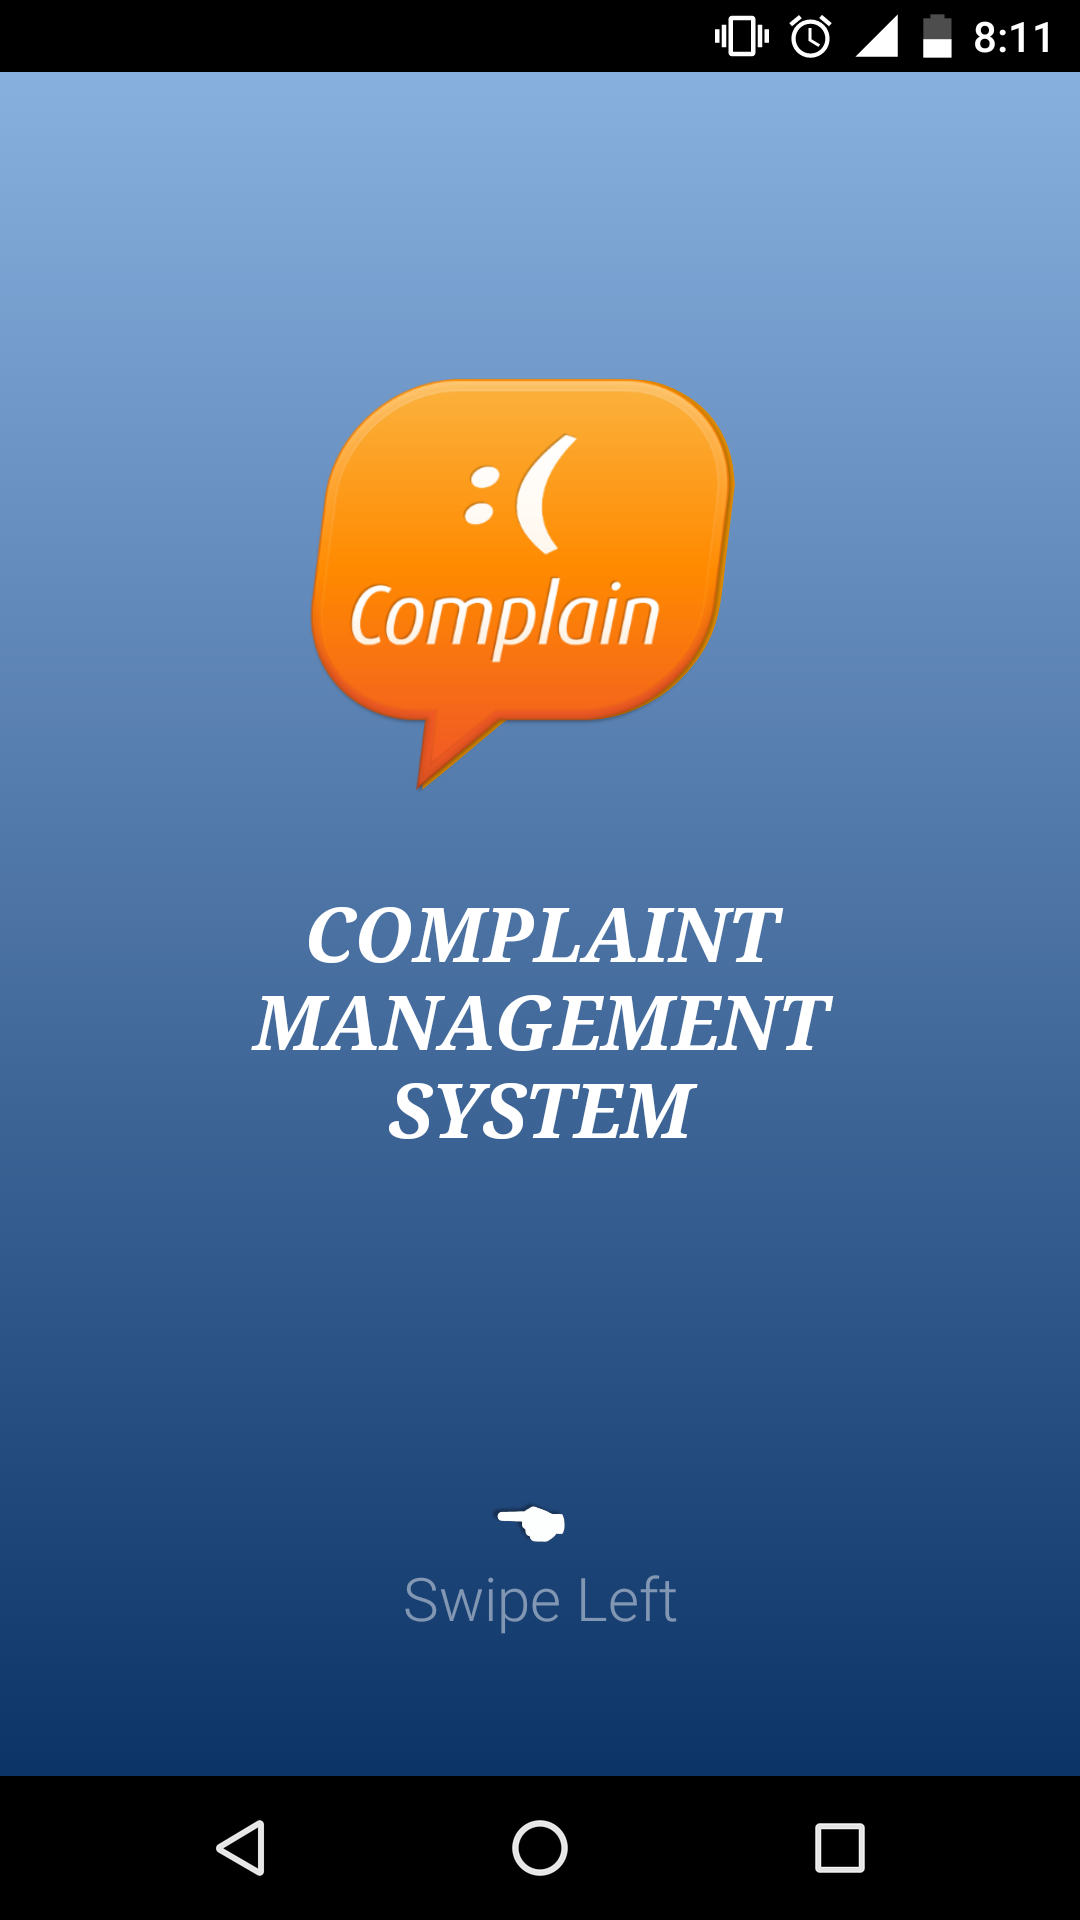
\includegraphics[width=10cm]{splash.png} \\
		% 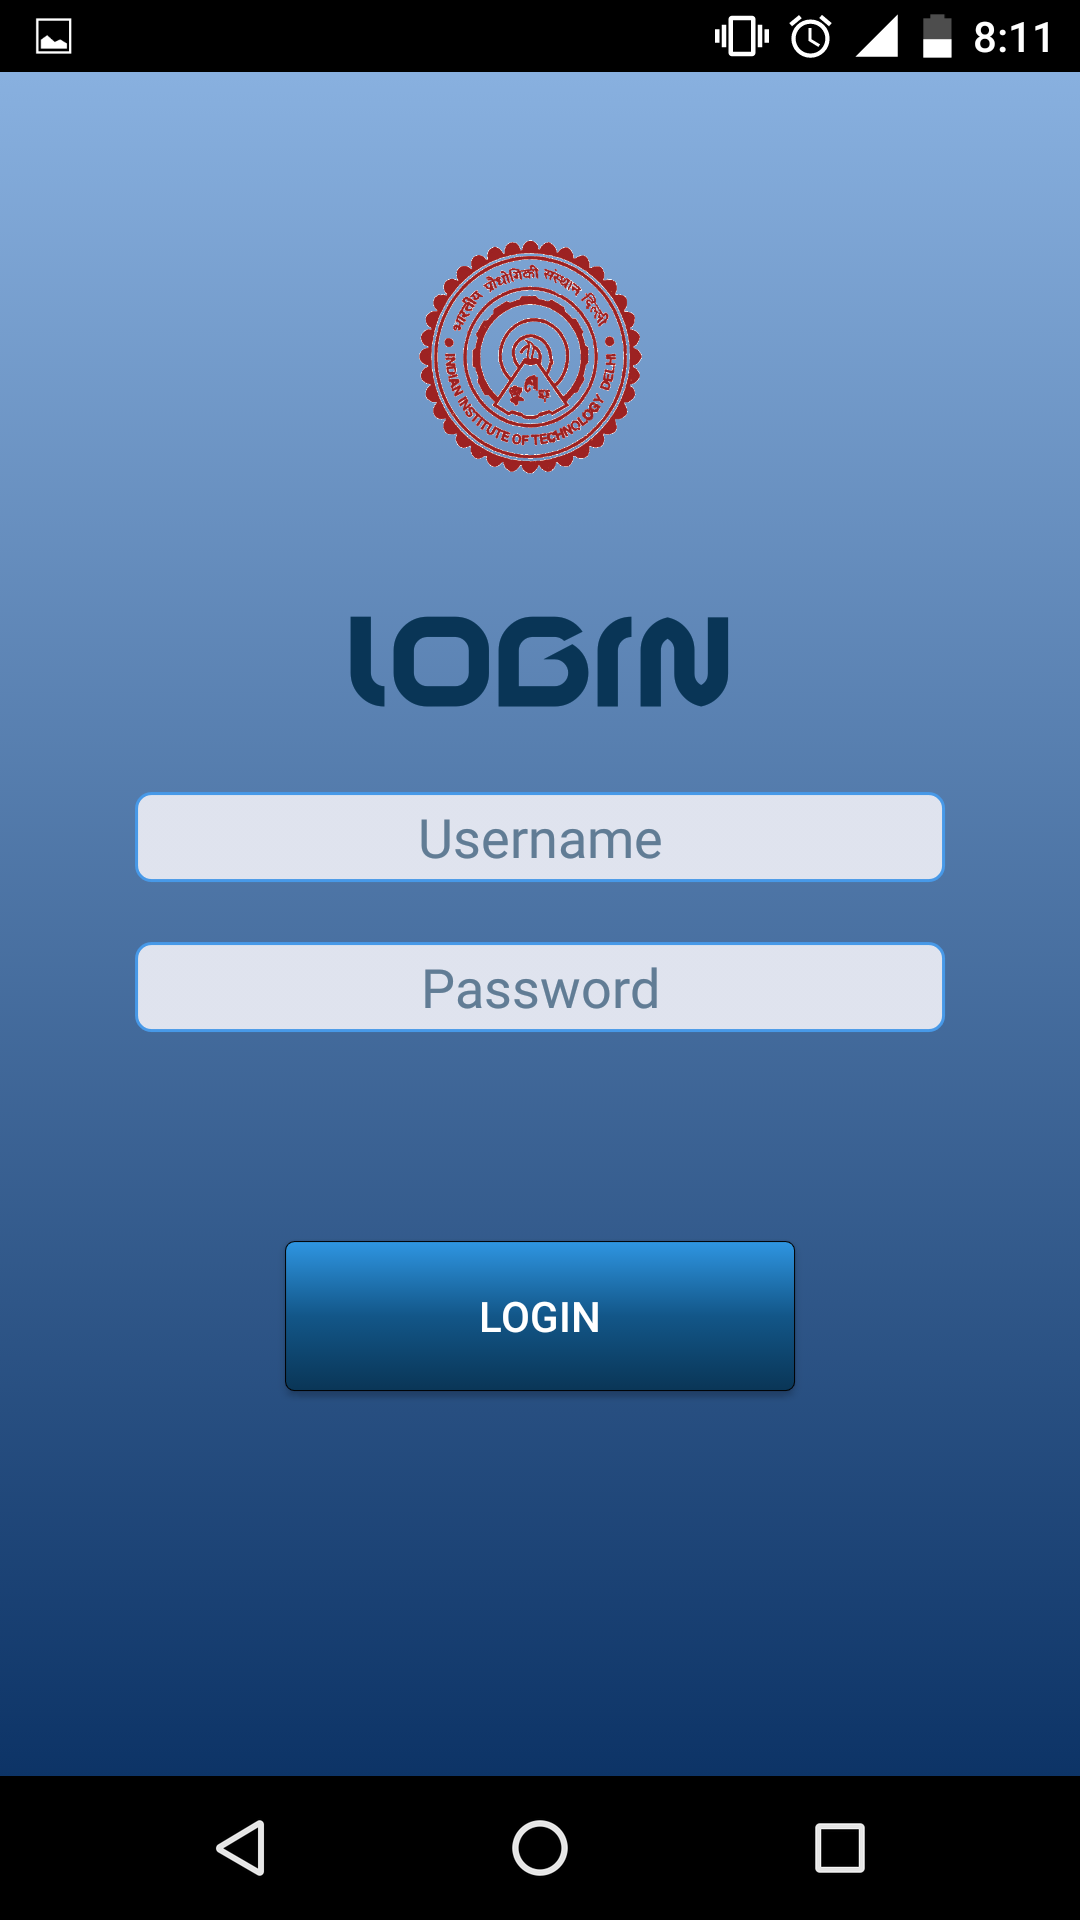
\includegraphics[width=10cm]{loginui.png} \\
		% \includegraphics{PComplaints.png} \\
		% \includegraphics{incomplaint.png} \\

	\section{Features}
		\subsection{Individual Complaints}
		\begin{itemize}
		\item The end user's complaint will be visible to the concerned authority only.
		\item Once the complaint is addressed,the user should be able to mark it as resolved
		\item The user can mark the complaint as resolved or take the complaint to the higher authority
		\end{itemize}
			\subsubsection{Options for the user}
				The person filing the complaint can fill in the following options:
				\begin{enumerate}
					\item Name
					\item Entry Number or Employee Number
					\item Phone Number
					\item Complain category
					\item Address/Hostel Name
					\item Content of the Complain
					\item Extra details
				\end{enumerate}
			\subsubsection{Options for the receiver}
				\begin{enumerate}
					\item See all details
					\item Request user to mark as completed
					\item Take to higher authority
				\end{enumerate}
			\subsubsection{Follow up options}
				\begin{enumerate}
					\item Mark the complain as completed
					\item Take to higher authority
				\end{enumerate}
			\subsubsection{Complaint Categories}
				\begin{enumerate}
					\item Room Maintenece
					\item Student Counselling Services
					\item BSW 
					\item Academic
				\end{enumerate}
		\subsection{Hostel Level Complaints}
		\begin{itemize}
		\item The end user's complaint would be visible to all the hostel residents who will be affected by the complaint.
		\item The concerned authority would have the right to mark the complaint as resolved.
		\item The complaint will be referred to a higher authority in a hierarchical order if 
			\begin{enumerate}
			\item Authority has marked the complaint as resolved but majority of users are not satisfied
			\item The time taken to resolve the complaint has exceeded a given time
			\end{enumerate}
		\item The Warden will be the highest authority.Veto powers will be given to the Warden
		\end{itemize}
			\subsubsection{User Options}
				\begin{enumerate}
					\item Name or Anonymous
					\item Entry Number or Anonymous 
					\item Phone Number or Anonymous
					\item Complain category
					\item Contents
					\item Additional Information
				\end{enumerate}
			\subsubsection{Other's Options}
				\begin{enumerate}
					\item People can Upvote, Downvote or be neutral to the complain.
					\item If the problem is not resolved in 7 days according to the majority, then the complain gets sent to the higher authority.
					\item People can add comments to the complain.
				\end{enumerate}
			\subsubsection{Receiver's Options}
				\begin{enumerate}
					\item Mark as resolved.
					\item Send to higher authority
				\end{enumerate}
			\subsubsection{Follow Up options}
				\begin{enumerate}
					\item Mark as resolved based on majority
					\item Send to higher authority based on majority
				\end{enumerate}
			\subsubsection{Complaint Categories}
				\begin{enumerate}
					\item Mess
					\item Maintenence
					\item Sports
					\item BSW
					\item Cultural Clubs
				\end{enumerate}
		\subsection{Institute Level Complaints}
		\begin{itemize}
		\item The end user's complaint would be visible to all the institute residents who will be affected by the complaint.
		\item The concerned authority would have the right to mark the complaint as resolved.
		\item The complaint will be referred to a higher authority in a hierarchical order if 
			\begin{enumerate}
			\item Authority has marked the complaint as resolved but majority of the users are not satisfied
			\item The time taken to resolve the complaint has exceeded a given time 
			\end{enumerate}
		\item The Concerned Dean will be the highest authority possessing Veto powers 
		\end{itemize}
			\subsubsection{User Options}
				\begin{enumerate}
					\item Name or Anonymous
					\item Entry Number or Anonymous 
					\item Phone Number or Anonymous
					\item Complain category
					\item Contents
					\item Additional Information
				\end{enumerate}
			\subsubsection{Other's Options}
				\begin{enumerate}
					\item People can Upvote, Downvote or be neutral to the complain.
					\item If the problem is not resolved in 7 days according to the majority, then the complain gets sent to the higher authority.
					\item People can add comments to the complain.
				\end{enumerate}
			\subsubsection{Receiver's Options}
				\begin{enumerate}
					\item Mark as resolved.
					\item Send to higher authority
				\end{enumerate}
			\subsubsection{Follow Up options}
				\begin{enumerate}
					\item Mark as resolved based on majority
					\item Send to higher authority based on majority
				\end{enumerate}
			\subsubsection{Complaint Categories}
				\begin{enumerate}
					\item General Infrastructure Faults
					\item Security
					\item Network Connectivity
					\item Cultural and Technical Clubs/Organisations
					\item Academic
				\end{enumerate}
	\section{Sub Components}
			\subsection{Server Back End}
				The back end has been divided into further sub components to facilitate the development process.
					%\subsubsection
					\subsubsection{Databases}
					\begin{table}[H]
\centering
\caption{User Database Table}
\label{my-label}
\begin{tabular}{|c|c|c|c|}
\hline
\textbf{S.No.} & \textbf{Fields} & \textbf{Type} & \textbf{Description}                                             \\ \hline
1              & Name            & String        & Name of the person                                               \\ \hline
2              & Unique Id       & String        & Entry Number for students or Employee Code for staff and faculty \\ \hline
3              & User Type       & Int           & Information regarding user being a student or staff or faculty   \\ \hline
4              & Contact Number  & String        & Phone Number                                                     \\ \hline
5              & Hostel          & String        & Hostel if any                                                    \\ \hline
6              & Other Details   & String        & Any other details                                                \\ \hline
7              & Password	 	 & String        & Password in hashed form                                          \\ \hline
8              & User Id                    & String        & Entry Number for students or Employee Code \\ \hline
9              & Hostel Preferences         & String        & Bit string to represent interest in Hostel activities            \\ \hline
10              & Institute Preferences & String        & Bit string to represent interest in Institute activities         \\ \hline
11             & Extra Preferences          & String        & Bit String to represent interest in Other activities             \\ \hline

\end{tabular}
\end{table}






\begin{table}[H]
\centering
\caption{Administrator Information}
\label{my-label}
\begin{tabular}{|c|c|c|c|}
\hline
\textbf{S.No.} & \textbf{Fields} & \textbf{Type} & \textbf{Description}                                             \\ \hline
1              & User Id         & String        & Unique user id \\ \hline
2              & Complaint Area  & Int           & Integer code for complaint area                                  \\ \hline
3              & Level           & Int           & Priority level for person                                        \\ \hline
4              & Description     & String        & Extra information                                                \\ \hline
5 				& Hostel Id  & Int & ID of hostel if any \\ \hline
\end{tabular}
\end{table}



\begin{table}[H]
\centering
\caption{Responses to a Complaint}
\label{my-label}
\begin{tabular}{|c|c|c|c|}
\hline
\textbf{S.No.} & \textbf{Fields} & \textbf{Type} & \textbf{Description}                                             \\ \hline
1              & User Id         & String        & Entry Number for students or Employee Code for staff and faculty \\ \hline
2              & Complaint Id    & Int           & Integer code for complaint area                                  \\ \hline
3              & Response         & Int           & Int corresponding to Upvote, Downvote or being neutral           \\ \hline
\end{tabular}
\end{table}


\begin{table}[H]
\centering
\caption{Hostel Mapping}
\label{my-label}
\begin{tabular}{|c|c|c|c|}
\hline
\textbf{S.No.} & \textbf{Fields} & \textbf{Type} & \textbf{Description} \\ \hline
1              & Hostel Id       & Int           & Integer for a hostel \\ \hline
2              & Hostel Name     & String        & String for hostel    \\ \hline
\end{tabular}
\end{table}



\begin{table}[H]
\centering
\caption{Complaint Category Mapping}
\label{my-label}
\begin{tabular}{|c|c|c|c|}
\hline
\textbf{S.No.} & \textbf{Fields}      & \textbf{Type} & \textbf{Description}             \\ \hline
1              & Category Id          & Int           & Integer for a complaint category \\ \hline
2              & Category Description & String        & String for a complaint category  \\ \hline
\end{tabular}
\end{table}


\begin{table}[H]
\centering
\caption{Comments on a complaint}
\label{my-label}
\begin{tabular}{|c|c|c|c|}
\hline
\textbf{S.No.} & \textbf{Fields} & \textbf{Type} & \textbf{Description}    \\ \hline
1              & Complaint Id    & String        & Unique Id for Complaint \\ \hline
2              & User Id         & String        & Unique User Id          \\ \hline
3              & Description     & String        & Complaint comment       \\ \hline
4              & Time Stamp      & Time          & Time of Comment         \\ \hline
5              & Anonymous      & Boolean          & Whether user is anonymous         \\ \hline
\end{tabular}
\end{table}


\begin{table}[H]
\centering
\caption{Complaint User Mapping}
\label{my-label}
\begin{tabular}{|c|c|c|c|}
\hline
\textbf{S.No.} & \textbf{Fields} & \textbf{Type} & \textbf{Description}    \\ \hline
1              & Complaint Id    & String        & Unique Id for Complaint \\ \hline
2              & User Id         & String        & Unique User Id          \\ \hline
\end{tabular}
\end{table}



\begin{table}[H]
\centering
\caption{Notifications}
\label{my-label}
\begin{tabular}{|c|c|c|c|}
\hline
\textbf{S.No.} & \textbf{Fields} & \textbf{Type} & \textbf{Description}    \\ \hline
1              & Complaint Id    & String        & Unique Id for Complaint \\ \hline
2              & From User Id    & String        & Unique User Id          \\ \hline
3              & To User Id      & String        & Unique User Id          \\ \hline
4              & Description     & String        & Content of notifcation  \\ \hline
5              & Seen            & Boolean       & Marked as seen or not   \\ \hline
\end{tabular}
\end{table}


\begin{table}[H]
\centering
\caption{User Satisfaction Response}
\label{my-label}
\begin{tabular}{|c|c|c|c|}
\hline
\textbf{S.No.} & \textbf{Fields} & \textbf{Type} & \textbf{Description}                                             \\ \hline
1              & User Id         & String        & Entry Number for students or Employee Code for staff and faculty \\ \hline
2              & Complaint Id    & Int           & Integer code for complaint area                                  \\ \hline
3              & Response         & Int           & Int corresponding to Satisfied or not 				           \\ \hline
\end{tabular}
\end{table}



\begin{table}[H]
\centering
\caption{Individual Complaint}
\label{my-label}
\begin{tabular}{|c|c|c|c|}
\hline
\textbf{S.No.} & \textbf{Fields}     & \textbf{Type} & \textbf{Description}                            \\ \hline
1              & Complaint Id        & String        & Unique Id for Complaint                         \\ \hline
2              & User Id             & String        & Unique User Id                                  \\ \hline
3              & Complaint Type      & Int           & Complaint category                              \\ \hline
4              & Complaint Content   & String        & Content of complaint                            \\ \hline
5              & Extra Info          & Image         & Upload a photo                                  \\ \hline
6              & Admin Id            & String        & Id of person assigned                           \\ \hline
7              & Time Stamp          & Time          & Time of filing the complaint                    \\ \hline
8              & Resolved            & Boolean       & Resolved or Not                                 \\ \hline
9              & Mark for resolution & Boolean       & Option for complaint addressee to seek approval \\ \hline
10             & Comment             & String        & Any comments                                    \\ \hline
11             & Previous Id         & Int           & Previous complaint id if any                    \\ \hline
\end{tabular}
\end{table}

\begin{table}[H]
\centering
\caption{Hostel Level Complaint}
\label{my-label}
\begin{tabular}{|c|c|c|c|}
\hline
\textbf{S.No.} & \textbf{Fields}     & \textbf{Type} & \textbf{Description}                            \\ \hline
1              & Complaint Id        & String        & Unique Id for Complaint                         \\ \hline
2              & User Id             & String        & Unique User Id                    \\ \hline
3              & Complaint Type      & Int           & Complaint category                              \\ \hline
4              & Complaint Content   & String        & Content of complaint                            \\ \hline
5              & Extra Info          & Image         & Upload a photo                                  \\ \hline
6              & Admin Id            & String        & Id of person assigned                           \\ \hline
7              & Time Stamp          & Time          & Time of filing the complaint                    \\ \hline
8              & Resolved            & Boolean       & Resolved or Not                                 \\ \hline
9              & Mark for resolution & Boolean       & Option for complaint addressee to seek approval \\ \hline
10             & Comment             & String        & Any comments                                    \\ \hline
11             & Previous Id         & Int           & Previous complaint id if any                    \\ \hline
12             & Hostel              & Int           & Hostel Id                                       \\ \hline
13			& Anonymous 		& Boolean &  Anonymous or not \\ \hline
14              & Number of Up-votes      & Int           & Number of Up-votes                           \\ \hline
15             & Number of Down-votes    & Int           & Number of Down-votes                         \\ \hline
16              & Number of Neutrals     & Int           & Number of Neutral people                    \\ \hline
17              & Number of Satisfied    & Int           & Number of people satisfied                  \\ \hline
18              & Number of Dissatisfied & Int           & Number of people dissatisfied with solution \\ \hline

\end{tabular}
\end{table}

\begin{table}[H]
\centering
\caption{Institute Level Complaint}
\label{my-label}
\begin{tabular}{|c|c|c|c|}
\hline
\textbf{S.No.} & \textbf{Fields}     & \textbf{Type} & \textbf{Description}                            \\ \hline
1              & Complaint Id        & String        & Unique Id for Complaint                         \\ \hline
2              & User Id             & String        & Unique User ID 				                     \\ \hline
3              & Complaint Type      & Int           & Complaint category                              \\ \hline
4              & Complaint Content   & String        & Content of complaint                            \\ \hline
5              & Extra Info          & File         & Upload a photo                                  \\ \hline
6              & Admin Id            & String        & Id of person assigned                           \\ \hline
7              & Time Stamp          & Time          & Time of filing the complaint                    \\ \hline
8              & Resolved            & Boolean       & Resolved or Not                                 \\ \hline
9              & Mark for resolution & Boolean       & Option for complaint addressee to seek approval \\ \hline
10             & Comment             & String        & Any comments                                    \\ \hline
11             & Previous Id         & Int           & Previous complaint id if any                    \\ \hline
12			& Anonymous 		& Boolean &  Anonymous or not \\ \hline
13              & Number of Up-votes      & Int           & Number of Up-votes                           \\ \hline
14              & Number of Down-votes    & Int           & Number of Down-votes                         \\ \hline
15              & Number of Neutrals     & Int           & Number of Neutral people                    \\ \hline
16              & Number of Satisfied    & Int           & Number of people satisfied                  \\ \hline
17              & Number of Dissatisfied & Int           & Number of people dissatisfied with solution \\ \hline

\end{tabular}
\end{table}

			\subsection{Network APIs}
				The following API's will be provided:
				(TODO: Separation of POST/GET)
				\begin{enumerate}
					\item \textbf{Login} \\
						URL: \url{/default/login.json?userid=<username>&password=<password>}  \\
						Returns: JSON object with Success/Failure and UserDetails
					\item \textbf{Logout} \\
						URL: \url{/default/logout.json} \\
						Returns: JSON object with Success/Failure
					\item \textbf{Change Password} \\
						URL: \url{/default/change_pass.json&password=<password>} \\
						Returns: JSON object with Success/Failure TODO: make it post	
					\item \textbf{Get Notifications} \\
						URL: \url{/default/notifications.json} \\
						Returns: JSON object containing list of all notifications. 
						A notification will be a TODO 
					\item \textbf{Get Preferences} \\
						URL: \url{/user/preferences.json} \\
						Returns: JSON object containing bitstrings of preferences and corresponding preference areas.
					\item \textbf{Set Preferences} \\
						URL: \url{/user/update_preferences.json?hostel=<hostel_pref>&institute=<insti_pref>&extra=<extra_pref>} \\
						Returns:  JSON object containing updated bitstrings and corresponding preference areas.
					\item \textbf{Get Administrator} \\
						URL: \url{/admin/get_admin.json?complian_area=<Complain>&level=<level>&Hostel=<hostel_id>}\\
						Returns:  JSON object containing  the administrator of a Complaint at a particular level
					\item \textbf{Get Response} \\
						URL: \url{/complaint/get_user_response.json?complian_id=<Complain>}\\
						Returns:  JSON object containing the response of a user to a public complaint 
					\item \textbf{Set Response} \\
						URL: \url{/complaint/set_user_response.json?complian_id=<Complain>&Response=<response>}\\
						Returns:   JSON object with Success/Failure.Sets the response of a user to a public complaint 
					\item \textbf{Complain Category Mapping} \\
						URL: \url{/complaint/get_desc.json?category_id=<cat>}\\
						Returns:   JSON object containing the category description 
					\item \textbf{Hostel Mapping} \\
						URL: \url{/default/get_hostel.json?hostel_id=<hos_id>}\\
						Returns:  JSON object containing the Hostel,ID pair 
					\item \textbf{Get Comment} \\
						URL: \url{/complaint/get_comments.json?complain_id=<id>}\\
						Returns:  JSON object containing all the comments on the thread to a complain
					\item \textbf{Post Comment} \\
						URL: \url{/complaint/post_comments.json?complain_id=<id>}\\
						Returns: JSON Success Response on posting a comment on the thread to a complain
					\item \textbf{Get Notification} \\
						URL: \url{/notification/get_noti.json}\\
						Returns: JSON object containing the set of notifications concerning the user
					\item \textbf{Set Notification Status} \\
						URL: \url{/notification/set_noti_status.json??compliant_id=<complain_id>}\\
						Returns: JSON object with Success/Failure.Sets the seen/unseen status of the user
% We can change the controller for the following API's but i m putting it in the complaint controller only
					\item \textbf{Get User Satisfaction} \\
						URL: \url{/complaint/get_user_satus.json?compliant_id=<complain_id>}\\
						Returns: JSON object containing the user's satisfaction after the complaint is resolved
					\item \textbf{Update user response} \\
						URL: \url{/complaint/put_user_satus.json?compliant_id=<complain_id>&response<bool>}\\
						Returns: JSON object with Success/Failure.Sets the user's satisfaction after the complaint is resolved
					\item \textbf{Add Complaint} \\
						URL: \url{/complaint_data/add_complaint.json?compliant_type=<type>&Complaint_content=<content>&extra_info=<file>&anonymous=<bool_anon>}\\
						Returns: JSON object with Success/Failure.Adds a complaint to the database
					\item \textbf{Edit Complaint} \\
						URL: \url{/complaint_data/edit_complaint.json?complaint_id=<id>&compliant_type=<type>&Complaint_content=<content>&extra_info=<file>&boolean_remove=<remove>&anonymous=<bool_anon>}\\
					% remove = true means we have to delete the complaint
						Returns: Edits an existing complaint in the database
					\item \textbf{Send to Higher Authority} \\
						URL: \url{/complaint/hig_auth.json?complaint_id=<id>}\\
						Returns: Sends the complaint to Higher Authority
					\item \textbf{Get all Complaints}
						URL: \url{/complaint_data/get_all.json}\\
						Returns: Return all the complaints concerning the user
					\item \textbf{Get Complaint Detail}	\\					
						URL: \url{/complaint_data/get_complaint_details.json?complaint_id=<id>}\\
						Returns: JSON object containing the details of a complaint 
	% Admin_complaint will be the admin side controller
					\item \textbf{Get Complaints to be Addressed} \\	
						URL: \url{/admin_complaint/get_all_complaints.json}\\
						Returns: JSON object containing all the complaints to be addressed
					\item \textbf{Get Complainant Details} \\
						URL: \url{/admin_complaint/get_complainant.json?complaint_id=<id>}\\
						Returns: JSON object containing the Complainant's detail
					\item \textbf{Mark Approved} \\
						URL: \url{/admin_complaint/mark_resolved.json?Complaint_id=<id>&boolean_resolve=<bool_done>}\\
						Returns: JSON object with Success/Failure.Success in marking for the Complainant's Approval
					\item \textbf{Add Administrator's Comment} \\ 
						URL: \url{/admin_complaint/add_comment.json?complaint_id=<id>&desc=<description>}\\
						Returns: JSON object with Success/Failure.Success in marking for the Complainant's Approval
					\item \textbf{Take to Higher Authority} \\ 
						URL: \url{/admin_complaint/add_comment.json?complaint_id=<id>}\\
						Returns: JSON object with Success/Failure.Success in sending the complaint to higher authority
					\item \textbf{Add User} \\ 
						URL: \url{TODO: POST}\\
						Returns: Adding user to the database 
				\end{enumerate}
			\subsection{Further server tasks}
				\begin{enumerate}
					\item Crontab tasks will be used to schedule periodic events like database cleanup and sending complaints to higher authorities.
					\item Crontab will also be used to generate push notifications for devices.
				\end{enumerate}
			\subsection{Android App Front End}
				TODO: Nikhil

		\subsection{Android App Back End}
		\begin{itemize}
		\item Volley will be used to send requests and receive responses.
		\item A separate class will be used to maintain the Session Cookies.
		\begin{lstlisting}[language=Java, caption={App\_Cookie Class}]
class App_Cookie extends Application
{	
   	CookieManager cookieManage;
   	// Manages the Cookie Session for the Entire Application
	public:
 	public void onCreate() 
	{
       cookieManage = new CookieManager();
       CookieHandler.setDefault(cookieManage);
       super.onCreate();
   	};
};
		\end{lstlisting}

		\item TODO:Sh*** Pre****
\begin{lstlisting}[language=Java, caption={Persistent Login}]
EditText username, password;
public static final String AppPREFERENCES = "AppPrefs";
public static final String UserId = "userId";
SharedPreferences sharedpreferences;
public void check_logged_in()
{// Checks if the user is already logged.
 // If logged in, he is directed to the HomePage. 
 sharedpreferences = getSharedPreferences
				(AppPREFERENCES,Context.MODE_PRIVATE);
 SharedPreferences.Editor editor = sharedpreferences.edit();
 int user_id= sharedpreferences.getInt("userID", 0);
 if(user_id!=0) // User_id is zero, if none is logged in
 {   Intent i = new Intent(Login.this,HomePage.class);
     i.putExtra("userID",user_id);
     startActivity(i);
 // Logged in user is directed to his Home Page
 }
 return;
};
		\end{lstlisting}		
		\end{itemize}

	\section{Interaction amongst Sub Components}
		% \subsection{enumerate}
			\subsection{Android App}
			\subsection{API and Server}
			\begin{enumerate}
				\item Event flow diagram for user login \\
					\includegraphics[width=15cm]{Login.png} \\
				\item Event flow diagram for user adding a complaint. \\
					\includegraphics[width=\linewidth]{Complaint.png}
			\end{enumerate}
			\subsection{Internal Server}
				Event flow diagram for crontab scheduling. \\
					\includegraphics[width=\linewidth]{cron.png}
	
	\section{Testing Of Components}
		% \begin{enumerate}
			\subsection{Server and APIs}
				\begin{itemize}
					\item Unit testing will be used to check if the server and end points are working correctly.
					\item For each endpoint, stress testing will be done via python or bash scripts to verify that the APIs perform as expected in various situations.
				\end{itemize}
			\subsection{Android App}
				We will use the Unit Testing component of Android studio to test each class created in the app for correctness. By doing this we will ensure that no errors take place on the android app and the user has a bug free experience.
			\subsection{Overall Testing}
				We will use the app on our phones once it is ready to identify and squash any remaining bugs in the app or the server. 	
	\section{Extra Features}
		\begin{itemize}
			\item The scope of the Application will be extended to Web Clients
			\item Hierarchy of Authorities would be maintained for every Complaint Type and Category
			\item In public level complaints option to register complaint as anonymous would be provided
			\item Users would be allowed to select the categories that affect them.Only public level complaints related to these categories will be displayed to the user
			\item Notification would be marked seen/unseen
			\item Users will get option to mark as satisfactory/unsatisfactory after the complaint is resolved
			\item Users will be able to post comments in the thread related to the concerned complaint
			\item The admin has an option to make a phone call or send an email through the app to the person who lodged the complaint.
		\end{itemize}

	\section{Future Endeavors} 
		\begin{itemize} 
			\item Keep local cache of changes done, at mobile level and sync them with the global server as soon as Internet connectivity is supplied.
			\item To extend the scope of Application to Windows as well as iOS client.Same Networking API's will be used.
			\item Users to be synchronized into the database via their Kerberos ID
			\item View location in google map/instiapp
		\end{itemize}   
	\section{Source Code}
	The source code of the project is maintained in the following repository: \\
	\url{https://github.com/aditi741997/COP290_Assignment_2.git}
	\bibliographystyle{abbrv}
	\medskip
	\bibliography{references}
\end{document} 
